\documentclass[1p]{elsarticle_modified}
%\bibliographystyle{elsarticle-num}

%\usepackage[colorlinks]{hyperref}
%\usepackage{abbrmath_seonhwa} %\Abb, \Ascr, \Acal ,\Abf, \Afrak
\usepackage{amsfonts}
\usepackage{amssymb}
\usepackage{amsmath}
\usepackage{amsthm}
\usepackage{scalefnt}
\usepackage{amsbsy}
\usepackage{kotex}
\usepackage{caption}
\usepackage{subfig}
\usepackage{color}
\usepackage{graphicx}
\usepackage{xcolor} %% white, black, red, green, blue, cyan, magenta, yellow
\usepackage{float}
\usepackage{setspace}
\usepackage{hyperref}

\usepackage{tikz}
\usetikzlibrary{arrows}

\usepackage{multirow}
\usepackage{array} % fixed length table
\usepackage{hhline}

%%%%%%%%%%%%%%%%%%%%%
\makeatletter
\renewcommand*\env@matrix[1][\arraystretch]{%
	\edef\arraystretch{#1}%
	\hskip -\arraycolsep
	\let\@ifnextchar\new@ifnextchar
	\array{*\c@MaxMatrixCols c}}
\makeatother %https://tex.stackexchange.com/questions/14071/how-can-i-increase-the-line-spacing-in-a-matrix
%%%%%%%%%%%%%%%

\usepackage[normalem]{ulem}

\newcommand{\msout}[1]{\ifmmode\text{\sout{\ensuremath{#1}}}\else\sout{#1}\fi}
%SOURCE: \msout is \stkout macro in https://tex.stackexchange.com/questions/20609/strikeout-in-math-mode

\newcommand{\cancel}[1]{
	\ifmmode
	{\color{red}\msout{#1}}
	\else
	{\color{red}\sout{#1}}
	\fi
}

\newcommand{\add}[1]{
	{\color{blue}\uwave{#1}}
}

\newcommand{\replace}[2]{
	\ifmmode
	{\color{red}\msout{#1}}{\color{blue}\uwave{#2}}
	\else
	{\color{red}\sout{#1}}{\color{blue}\uwave{#2}}
	\fi
}

\newcommand{\Sol}{\mathcal{S}} %segment
\newcommand{\D}{D} %diagram
\newcommand{\A}{\mathcal{A}} %arc


%%%%%%%%%%%%%%%%%%%%%%%%%%%%%5 test

\def\sl{\operatorname{\textup{SL}}(2,\Cbb)}
\def\psl{\operatorname{\textup{PSL}}(2,\Cbb)}
\def\quan{\mkern 1mu \triangleright \mkern 1mu}

\theoremstyle{definition}
\newtheorem{thm}{Theorem}[section]
\newtheorem{prop}[thm]{Proposition}
\newtheorem{lem}[thm]{Lemma}
\newtheorem{ques}[thm]{Question}
\newtheorem{cor}[thm]{Corollary}
\newtheorem{defn}[thm]{Definition}
\newtheorem{exam}[thm]{Example}
\newtheorem{rmk}[thm]{Remark}
\newtheorem{alg}[thm]{Algorithm}

\newcommand{\I}{\sqrt{-1}}
\begin{document}

%\begin{frontmatter}
%
%\title{Boundary parabolic representations of knots up to 8 crossings}
%
%%% Group authors per affiliation:
%\author{Yunhi Cho} 
%\address{Department of Mathematics, University of Seoul, Seoul, Korea}
%\ead{yhcho@uos.ac.kr}
%
%
%\author{Seonhwa Kim} %\fnref{s_kim}}
%\address{Center for Geometry and Physics, Institute for Basic Science, Pohang, 37673, Korea}
%\ead{ryeona17@ibs.re.kr}
%
%\author{Hyuk Kim}
%\address{Department of Mathematical Sciences, Seoul National University, Seoul 08826, Korea}
%\ead{hyukkim@snu.ac.kr}
%
%\author{Seokbeom Yoon}
%\address{Department of Mathematical Sciences, Seoul National University, Seoul, 08826,  Korea}
%\ead{sbyoon15@snu.ac.kr}
%
%\begin{abstract}
%We find all boundary parabolic representation of knots up to 8 crossings.
%
%\end{abstract}
%\begin{keyword}
%    \MSC[2010] 57M25 
%\end{keyword}
%
%\end{frontmatter}

%\linenumbers
%\tableofcontents
%
\newcommand\colored[1]{\textcolor{white}{\rule[-0.35ex]{0.8em}{1.4ex}}\kern-0.8em\color{red} #1}%
%\newcommand\colored[1]{\textcolor{white}{ #1}\kern-2.17ex	\textcolor{white}{ #1}\kern-1.81ex	\textcolor{white}{ #1}\kern-2.15ex\color{red}#1	}

{\Large $\underline{10_{84}~(K10a_{50})}$}

\setlength{\tabcolsep}{10pt}
\renewcommand{\arraystretch}{1.6}
\vspace{1cm}\begin{tabular}{m{100pt}>{\centering\arraybackslash}m{274pt}}
\multirow{5}{120pt}{
	\centering
	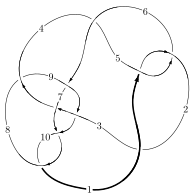
\includegraphics[width=112pt]{../../../GIT/diagram.site/Diagrams/png/168_10_84.png}\\
\ \ \ A knot diagram\footnotemark}&
\allowdisplaybreaks
\textbf{Linearized knot diagam} \\
\cline{2-2}
 &
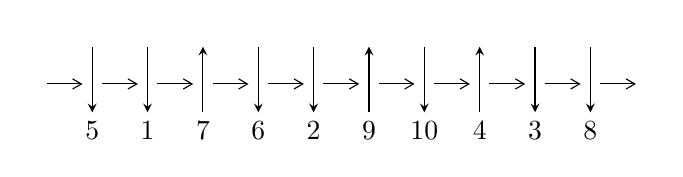
\begin{tikzpicture}[x=20pt, y=17pt]
	% nodes
	\node (C0) at (0, 0) {};
	\node (C1) at (1, 0) {};
	\node (C1U) at (1, +1) {};
	\node (C1D) at (1, -1) {5};

	\node (C2) at (2, 0) {};
	\node (C2U) at (2, +1) {};
	\node (C2D) at (2, -1) {1};

	\node (C3) at (3, 0) {};
	\node (C3U) at (3, +1) {};
	\node (C3D) at (3, -1) {7};

	\node (C4) at (4, 0) {};
	\node (C4U) at (4, +1) {};
	\node (C4D) at (4, -1) {6};

	\node (C5) at (5, 0) {};
	\node (C5U) at (5, +1) {};
	\node (C5D) at (5, -1) {2};

	\node (C6) at (6, 0) {};
	\node (C6U) at (6, +1) {};
	\node (C6D) at (6, -1) {9};

	\node (C7) at (7, 0) {};
	\node (C7U) at (7, +1) {};
	\node (C7D) at (7, -1) {10};

	\node (C8) at (8, 0) {};
	\node (C8U) at (8, +1) {};
	\node (C8D) at (8, -1) {4};

	\node (C9) at (9, 0) {};
	\node (C9U) at (9, +1) {};
	\node (C9D) at (9, -1) {3};

	\node (C10) at (10, 0) {};
	\node (C10U) at (10, +1) {};
	\node (C10D) at (10, -1) {8};
	\node (C11) at (11, 0) {};

	% arrows
	\draw[->,>={angle 60}]
	(C0) edge (C1) (C1) edge (C2) (C2) edge (C3) (C3) edge (C4) (C4) edge (C5) (C5) edge (C6) (C6) edge (C7) (C7) edge (C8) (C8) edge (C9) (C9) edge (C10) (C10) edge (C11) ;	\draw[->,>=stealth]
	(C1U) edge (C1D) (C2U) edge (C2D) (C3D) edge (C3U) (C4U) edge (C4D) (C5U) edge (C5D) (C6D) edge (C6U) (C7U) edge (C7D) (C8D) edge (C8U) (C9U) edge (C9D) (C10U) edge (C10D) ;
	\end{tikzpicture} \\
\hhline{~~} \\& 
\textbf{Solving Sequence} \\ \cline{2-2} 
 &
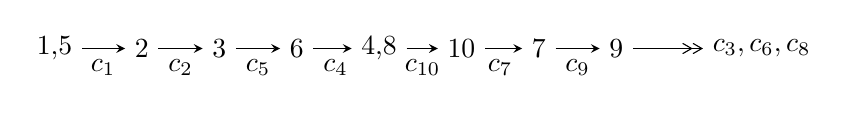
\begin{tikzpicture}[x=28pt, y=7pt]
	% node
	\node (A0) at (-1/8, 0) {1,5};
	\node (A1) at (1, 0) {2};
	\node (A2) at (2, 0) {3};
	\node (A3) at (3, 0) {6};
	\node (A4) at (65/16, 0) {4,8};
	\node (A5) at (41/8, 0) {10};
	\node (A6) at (49/8, 0) {7};
	\node (A7) at (57/8, 0) {9};
	\node (C1) at (1/2, -1) {$c_{1}$};
	\node (C2) at (3/2, -1) {$c_{2}$};
	\node (C3) at (5/2, -1) {$c_{5}$};
	\node (C4) at (7/2, -1) {$c_{4}$};
	\node (C5) at (37/8, -1) {$c_{10}$};
	\node (C6) at (45/8, -1) {$c_{7}$};
	\node (C7) at (53/8, -1) {$c_{9}$};
	\node (A8) at (9, 0) {$c_{3},c_{6},c_{8}$};

	% edge
	\draw[->,>=stealth]	
	(A0) edge (A1) (A1) edge (A2) (A2) edge (A3) (A3) edge (A4) (A4) edge (A5) (A5) edge (A6) (A6) edge (A7) ;
	\draw[->>,>={angle 60}]	
	(A7) edge (A8);
\end{tikzpicture} \\ 

\end{tabular} \\

\footnotetext{
The image of knot diagram is generated by the software ``\textbf{Draw programme}" developed by Andrew Bartholomew(\url{http://www.layer8.co.uk/maths/draw/index.htm\#Running-draw}), where we modified some parts for our purpose(\url{https://github.com/CATsTAILs/LinksPainter}).
}\phantom \\ \newline 
\centering \textbf{Ideals for irreducible components\footnotemark of $X_{\text{par}}$} 
 
\begin{align*}
I^u_{1}&=\langle 
-26695942110849 u^{43}+24221062450767 u^{42}+\cdots+146051535266254 b+143537280527879,\\
\phantom{I^u_{1}}&\phantom{= \langle  }-958891166678785 u^{43}+1195830341741191 u^{42}+\cdots+146051535266254 a+928016870112473,\\
\phantom{I^u_{1}}&\phantom{= \langle  }u^{44}-2 u^{43}+\cdots-5 u+1\rangle \\
I^u_{2}&=\langle 
b+1,\;a+2,\;u-1\rangle \\
\\
\end{align*}
\raggedright * 2 irreducible components of $\dim_{\mathbb{C}}=0$, with total 45 representations.\\
\footnotetext{All coefficients of polynomials are rational numbers. But the coefficients are sometimes approximated in decimal forms when there is not enough margin.}
\newpage
\renewcommand{\arraystretch}{1}
\centering \section*{I. $I^u_{1}= \langle -2.67\times10^{13} u^{43}+2.42\times10^{13} u^{42}+\cdots+1.46\times10^{14} b+1.44\times10^{14},\;-9.59\times10^{14} u^{43}+1.20\times10^{15} u^{42}+\cdots+1.46\times10^{14} a+9.28\times10^{14},\;u^{44}-2 u^{43}+\cdots-5 u+1 \rangle$}
\flushleft \textbf{(i) Arc colorings}\\
\begin{tabular}{m{7pt} m{180pt} m{7pt} m{180pt} }
\flushright $a_{1}=$&$\begin{pmatrix}1\\0\end{pmatrix}$ \\
\flushright $a_{5}=$&$\begin{pmatrix}0\\u\end{pmatrix}$ \\
\flushright $a_{2}=$&$\begin{pmatrix}1\\u^2\end{pmatrix}$ \\
\flushright $a_{3}=$&$\begin{pmatrix}- u^2+1\\u^2\end{pmatrix}$ \\
\flushright $a_{6}=$&$\begin{pmatrix}- u\\- u^3+u\end{pmatrix}$ \\
\flushright $a_{4}=$&$\begin{pmatrix}u^3\\u^5- u^3+u\end{pmatrix}$ \\
\flushright $a_{8}=$&$\begin{pmatrix}6.56543 u^{43}-8.18773 u^{42}+\cdots+35.0046 u-6.35404\\0.182784 u^{43}-0.165839 u^{42}+\cdots-0.0574672 u-0.982785\end{pmatrix}$ \\
\flushright $a_{10}=$&$\begin{pmatrix}6.55549 u^{43}-8.08325 u^{42}+\cdots+36.0390 u-5.60107\\0.268862 u^{43}-0.336643 u^{42}+\cdots+0.229869 u-1.06886\end{pmatrix}$ \\
\flushright $a_{7}=$&$\begin{pmatrix}-0.202656 u^{43}-0.625196 u^{42}+\cdots-1.87375 u-0.511274\\-0.827844 u^{43}+1.65839 u^{42}+\cdots-3.42533 u+0.827852\end{pmatrix}$ \\
\flushright $a_{9}=$&$\begin{pmatrix}4.95923 u^{43}-5.84946 u^{42}+\cdots+26.4222 u-4.00846\\-1.49853 u^{43}+1.58954 u^{42}+\cdots-9.24326 u+1.49850\end{pmatrix}$\\&\end{tabular}
\flushleft \textbf{(ii) Obstruction class $= -1$}\\~\\
\flushleft \textbf{(iii) Cusp Shapes $= -\frac{2627515223052688}{73025767633127} u^{43}+\frac{3096365063700750}{73025767633127} u^{42}+\cdots-\frac{11221793809688154}{73025767633127} u+\frac{2703461955268724}{73025767633127}$}\\~\\
\newpage\renewcommand{\arraystretch}{1}
\flushleft \textbf{(iv) u-Polynomials at the component}\newline \\
\begin{tabular}{m{50pt}|m{274pt}}
Crossings & \hspace{64pt}u-Polynomials at each crossing \\
\hline $$\begin{aligned}c_{1},c_{5}\end{aligned}$$&$\begin{aligned}
&u^{44}+2 u^{43}+\cdots+5 u+1
\end{aligned}$\\
\hline $$\begin{aligned}c_{2},c_{4}\end{aligned}$$&$\begin{aligned}
&u^{44}+14 u^{43}+\cdots- u+1
\end{aligned}$\\
\hline $$\begin{aligned}c_{3}\end{aligned}$$&$\begin{aligned}
&u^{44}+4 u^{43}+\cdots- u-1
\end{aligned}$\\
\hline $$\begin{aligned}c_{6}\end{aligned}$$&$\begin{aligned}
&u^{44}+7 u^{43}+\cdots-2 u+2
\end{aligned}$\\
\hline $$\begin{aligned}c_{7},c_{10}\end{aligned}$$&$\begin{aligned}
&u^{44}-2 u^{43}+\cdots-5 u-1
\end{aligned}$\\
\hline $$\begin{aligned}c_{8}\end{aligned}$$&$\begin{aligned}
&u^{44}-2 u^{43}+\cdots-17 u-11
\end{aligned}$\\
\hline $$\begin{aligned}c_{9}\end{aligned}$$&$\begin{aligned}
&u^{44}-4 u^{43}+\cdots-21 u+1
\end{aligned}$\\
\hline
\end{tabular}\\~\\
\newpage\renewcommand{\arraystretch}{1}
\flushleft \textbf{(v) Riley Polynomials at the component}\newline \\
\begin{tabular}{m{50pt}|m{274pt}}
Crossings & \hspace{64pt}Riley Polynomials at each crossing \\
\hline $$\begin{aligned}c_{1},c_{5}\end{aligned}$$&$\begin{aligned}
&y^{44}-14 y^{43}+\cdots+y+1
\end{aligned}$\\
\hline $$\begin{aligned}c_{2},c_{4}\end{aligned}$$&$\begin{aligned}
&y^{44}+34 y^{43}+\cdots+137 y+1
\end{aligned}$\\
\hline $$\begin{aligned}c_{3}\end{aligned}$$&$\begin{aligned}
&y^{44}+6 y^{43}+\cdots+y+1
\end{aligned}$\\
\hline $$\begin{aligned}c_{6}\end{aligned}$$&$\begin{aligned}
&y^{44}-9 y^{43}+\cdots-40 y+4
\end{aligned}$\\
\hline $$\begin{aligned}c_{7},c_{10}\end{aligned}$$&$\begin{aligned}
&y^{44}-26 y^{43}+\cdots-71 y+1
\end{aligned}$\\
\hline $$\begin{aligned}c_{8}\end{aligned}$$&$\begin{aligned}
&y^{44}-42 y^{43}+\cdots-2995 y+121
\end{aligned}$\\
\hline $$\begin{aligned}c_{9}\end{aligned}$$&$\begin{aligned}
&y^{44}-38 y^{43}+\cdots-123 y+1
\end{aligned}$\\
\hline
\end{tabular}\\~\\
\newpage\flushleft \textbf{(vi) Complex Volumes and Cusp Shapes}
$$\begin{array}{c|c|c}  
\text{Solutions to }I^u_{1}& \I (\text{vol} + \sqrt{-1}CS) & \text{Cusp shape}\\
 \hline 
\begin{aligned}
u &= -0.927602 + 0.226351 I \\
a &= -0.224310 - 0.062924 I \\
b &= -0.115105 + 0.911207 I\end{aligned}
 & -1.13001 + 3.88298 I & -6.50680 - 7.75927 I \\ \hline\begin{aligned}
u &= -0.927602 - 0.226351 I \\
a &= -0.224310 + 0.062924 I \\
b &= -0.115105 - 0.911207 I\end{aligned}
 & -1.13001 - 3.88298 I & -6.50680 + 7.75927 I \\ \hline\begin{aligned}
u &= \phantom{-}0.778786 + 0.710214 I \\
a &= \phantom{-}1.43805 - 0.91909 I \\
b &= -1.049480 + 0.821846 I\end{aligned}
 & \phantom{-}0.040125 + 0.820231 I & -5.81896 - 3.03229 I \\ \hline\begin{aligned}
u &= \phantom{-}0.778786 - 0.710214 I \\
a &= \phantom{-}1.43805 + 0.91909 I \\
b &= -1.049480 - 0.821846 I\end{aligned}
 & \phantom{-}0.040125 - 0.820231 I & -5.81896 + 3.03229 I \\ \hline\begin{aligned}
u &= -0.927070 + 0.063011 I \\
a &= -1.49031 - 0.50021 I \\
b &= -1.37113 + 0.48363 I\end{aligned}
 & -4.92583 + 1.73663 I & -14.9087 - 4.1335 I \\ \hline\begin{aligned}
u &= -0.927070 - 0.063011 I \\
a &= -1.49031 + 0.50021 I \\
b &= -1.37113 - 0.48363 I\end{aligned}
 & -4.92583 - 1.73663 I & -14.9087 + 4.1335 I \\ \hline\begin{aligned}
u &= -0.658922 + 0.846151 I \\
a &= -0.183634 - 0.593747 I \\
b &= \phantom{-}0.865773 + 0.460561 I\end{aligned}
 & \phantom{-}3.70844 - 0.99499 I & \phantom{-}0.63089 + 2.41468 I \\ \hline\begin{aligned}
u &= -0.658922 - 0.846151 I \\
a &= -0.183634 + 0.593747 I \\
b &= \phantom{-}0.865773 - 0.460561 I\end{aligned}
 & \phantom{-}3.70844 + 0.99499 I & \phantom{-}0.63089 - 2.41468 I \\ \hline\begin{aligned}
u &= \phantom{-}0.878177 + 0.660456 I \\
a &= \phantom{-}0.670319 + 1.230810 I \\
b &= -1.59639 + 0.09563 I\end{aligned}
 & -1.82200 - 2.55706 I & -9.50147 + 2.98004 I \\ \hline\begin{aligned}
u &= \phantom{-}0.878177 - 0.660456 I \\
a &= \phantom{-}0.670319 - 1.230810 I \\
b &= -1.59639 - 0.09563 I\end{aligned}
 & -1.82200 + 2.55706 I & -9.50147 - 2.98004 I\\
 \hline 
 \end{array}$$\newpage$$\begin{array}{c|c|c}  
\text{Solutions to }I^u_{1}& \I (\text{vol} + \sqrt{-1}CS) & \text{Cusp shape}\\
 \hline 
\begin{aligned}
u &= -0.840203 + 0.731796 I \\
a &= \phantom{-}0.53742 + 1.70678 I \\
b &= -0.912754 - 0.201576 I\end{aligned}
 & \phantom{-}1.40942 + 2.09852 I & -2.80453 - 11.50069 I \\ \hline\begin{aligned}
u &= -0.840203 - 0.731796 I \\
a &= \phantom{-}0.53742 - 1.70678 I \\
b &= -0.912754 + 0.201576 I\end{aligned}
 & \phantom{-}1.40942 - 2.09852 I & -2.80453 + 11.50069 I \\ \hline\begin{aligned}
u &= \phantom{-}0.772905 + 0.818777 I \\
a &= \phantom{-}0.33712 - 1.68078 I \\
b &= \phantom{-}0.254394 + 1.136870 I\end{aligned}
 & \phantom{-}5.49636 + 2.42871 I & \phantom{-0.000000 } 0. - 2.25678 I \\ \hline\begin{aligned}
u &= \phantom{-}0.772905 - 0.818777 I \\
a &= \phantom{-}0.33712 + 1.68078 I \\
b &= \phantom{-}0.254394 - 1.136870 I\end{aligned}
 & \phantom{-}5.49636 - 2.42871 I & \phantom{-0.000000 -}0. + 2.25678 I \\ \hline\begin{aligned}
u &= \phantom{-}0.709073 + 0.883385 I \\
a &= -0.840026 + 0.862508 I \\
b &= \phantom{-}1.27066 - 0.62408 I\end{aligned}
 & \phantom{-}2.27409 + 8.60569 I & -2.63926 - 4.58190 I \\ \hline\begin{aligned}
u &= \phantom{-}0.709073 - 0.883385 I \\
a &= -0.840026 - 0.862508 I \\
b &= \phantom{-}1.27066 + 0.62408 I\end{aligned}
 & \phantom{-}2.27409 - 8.60569 I & -2.63926 + 4.58190 I \\ \hline\begin{aligned}
u &= -1.117850 + 0.238085 I \\
a &= \phantom{-}1.25957 + 0.83369 I \\
b &= \phantom{-}1.277770 - 0.452951 I\end{aligned}
 & -5.29949 + 8.62766 I & -9.10597 - 7.54655 I \\ \hline\begin{aligned}
u &= -1.117850 - 0.238085 I \\
a &= \phantom{-}1.25957 - 0.83369 I \\
b &= \phantom{-}1.277770 + 0.452951 I\end{aligned}
 & -5.29949 - 8.62766 I & -9.10597 + 7.54655 I \\ \hline\begin{aligned}
u &= -0.902384 + 0.723912 I \\
a &= -0.42622 - 3.07845 I \\
b &= -0.993100 + 0.182802 I\end{aligned}
 & \phantom{-}1.21777 + 3.45181 I & \phantom{-0.000000 -}0. + 7.88863 I \\ \hline\begin{aligned}
u &= -0.902384 - 0.723912 I \\
a &= -0.42622 + 3.07845 I \\
b &= -0.993100 - 0.182802 I\end{aligned}
 & \phantom{-}1.21777 - 3.45181 I & \phantom{-0.000000 } 0. - 7.88863 I\\
 \hline 
 \end{array}$$\newpage$$\begin{array}{c|c|c}  
\text{Solutions to }I^u_{1}& \I (\text{vol} + \sqrt{-1}CS) & \text{Cusp shape}\\
 \hline 
\begin{aligned}
u &= \phantom{-}0.940648 + 0.702120 I \\
a &= -0.12431 + 2.40011 I \\
b &= -1.20650 - 0.83342 I\end{aligned}
 & -0.45271 - 6.24747 I & -7.31920 + 8.44159 I \\ \hline\begin{aligned}
u &= \phantom{-}0.940648 - 0.702120 I \\
a &= -0.12431 - 2.40011 I \\
b &= -1.20650 + 0.83342 I\end{aligned}
 & -0.45271 + 6.24747 I & -7.31920 - 8.44159 I \\ \hline\begin{aligned}
u &= \phantom{-}1.18227\phantom{ +0.000000I} \\
a &= \phantom{-}1.12361\phantom{ +0.000000I} \\
b &= \phantom{-}0.834518\phantom{ +0.000000I}\end{aligned}
 & -2.71479\phantom{ +0.000000I} & \phantom{-}5.71830\phantom{ +0.000000I} \\ \hline\begin{aligned}
u &= \phantom{-}0.802912 + 0.142507 I \\
a &= \phantom{-}0.916574 + 0.518690 I \\
b &= -0.174142 - 0.024221 I\end{aligned}
 & -1.40557 - 0.34934 I & -7.47293 + 0.48118 I \\ \hline\begin{aligned}
u &= \phantom{-}0.802912 - 0.142507 I \\
a &= \phantom{-}0.916574 - 0.518690 I \\
b &= -0.174142 + 0.024221 I\end{aligned}
 & -1.40557 + 0.34934 I & -7.47293 - 0.48118 I \\ \hline\begin{aligned}
u &= \phantom{-}0.812067\phantom{ +0.000000I} \\
a &= -6.68009\phantom{ +0.000000I} \\
b &= -1.03778\phantom{ +0.000000I}\end{aligned}
 & -2.95636\phantom{ +0.000000I} & \phantom{-}47.1560\phantom{ +0.000000I} \\ \hline\begin{aligned}
u &= \phantom{-}0.098222 + 0.805268 I \\
a &= -0.628805 - 0.691139 I \\
b &= \phantom{-}1.121430 + 0.435398 I\end{aligned}
 & -1.20700 - 5.24815 I & -2.80453 + 6.18731 I \\ \hline\begin{aligned}
u &= \phantom{-}0.098222 - 0.805268 I \\
a &= -0.628805 + 0.691139 I \\
b &= \phantom{-}1.121430 - 0.435398 I\end{aligned}
 & -1.20700 + 5.24815 I & -2.80453 - 6.18731 I \\ \hline\begin{aligned}
u &= \phantom{-}1.133010 + 0.369128 I \\
a &= \phantom{-}0.498144 - 0.725878 I \\
b &= \phantom{-}1.113320 - 0.253728 I\end{aligned}
 & -4.55359 + 1.09231 I & -9.24999 - 5.05772 I \\ \hline\begin{aligned}
u &= \phantom{-}1.133010 - 0.369128 I \\
a &= \phantom{-}0.498144 + 0.725878 I \\
b &= \phantom{-}1.113320 + 0.253728 I\end{aligned}
 & -4.55359 - 1.09231 I & -9.24999 + 5.05772 I\\
 \hline 
 \end{array}$$\newpage$$\begin{array}{c|c|c}  
\text{Solutions to }I^u_{1}& \I (\text{vol} + \sqrt{-1}CS) & \text{Cusp shape}\\
 \hline 
\begin{aligned}
u &= -0.835443 + 0.852874 I \\
a &= -0.056114 + 0.817361 I \\
b &= \phantom{-}0.565371 - 0.419340 I\end{aligned}
 & \phantom{-}4.53169 + 2.82413 I & \phantom{-0.000000 } 0. - 4.92903 I \\ \hline\begin{aligned}
u &= -0.835443 - 0.852874 I \\
a &= -0.056114 - 0.817361 I \\
b &= \phantom{-}0.565371 + 0.419340 I\end{aligned}
 & \phantom{-}4.53169 - 2.82413 I & \phantom{-0.000000 -}0. + 4.92903 I \\ \hline\begin{aligned}
u &= -0.940979 + 0.796566 I \\
a &= -0.298082 - 0.266590 I \\
b &= \phantom{-}0.375731 + 0.414152 I\end{aligned}
 & \phantom{-}4.19341 + 3.30756 I & \phantom{-0.000000 } 0 \\ \hline\begin{aligned}
u &= -0.940979 - 0.796566 I \\
a &= -0.298082 + 0.266590 I \\
b &= \phantom{-}0.375731 - 0.414152 I\end{aligned}
 & \phantom{-}4.19341 - 3.30756 I & \phantom{-0.000000 } 0 \\ \hline\begin{aligned}
u &= \phantom{-}0.973933 + 0.757495 I \\
a &= -1.09792 + 1.17097 I \\
b &= \phantom{-}0.181664 - 1.203370 I\end{aligned}
 & \phantom{-}4.87682 - 8.33877 I & \phantom{-0.000000 -}0. + 7.62816 I \\ \hline\begin{aligned}
u &= \phantom{-}0.973933 - 0.757495 I \\
a &= -1.09792 - 1.17097 I \\
b &= \phantom{-}0.181664 + 1.203370 I\end{aligned}
 & \phantom{-}4.87682 + 8.33877 I & \phantom{-0.000000 } 0. - 7.62816 I \\ \hline\begin{aligned}
u &= -1.046830 + 0.731985 I \\
a &= \phantom{-}0.54736 + 1.47326 I \\
b &= \phantom{-}0.992978 - 0.410523 I\end{aligned}
 & \phantom{-}2.52892 + 6.89763 I & \phantom{-0.000000 } 0 \\ \hline\begin{aligned}
u &= -1.046830 - 0.731985 I \\
a &= \phantom{-}0.54736 - 1.47326 I \\
b &= \phantom{-}0.992978 + 0.410523 I\end{aligned}
 & \phantom{-}2.52892 - 6.89763 I & \phantom{-0.000000 } 0 \\ \hline\begin{aligned}
u &= \phantom{-}1.033090 + 0.762400 I \\
a &= \phantom{-}0.30235 - 2.16182 I \\
b &= \phantom{-}1.32116 + 0.62604 I\end{aligned}
 & \phantom{-}1.2704 - 14.7099 I & \phantom{-0.000000 } 0 \\ \hline\begin{aligned}
u &= \phantom{-}1.033090 - 0.762400 I \\
a &= \phantom{-}0.30235 + 2.16182 I \\
b &= \phantom{-}1.32116 - 0.62604 I\end{aligned}
 & \phantom{-}1.2704 + 14.7099 I & \phantom{-0.000000 } 0\\
 \hline 
 \end{array}$$\newpage$$\begin{array}{c|c|c}  
\text{Solutions to }I^u_{1}& \I (\text{vol} + \sqrt{-1}CS) & \text{Cusp shape}\\
 \hline 
\begin{aligned}
u &= -0.109387 + 0.546973 I \\
a &= \phantom{-}0.696572 + 1.005610 I \\
b &= \phantom{-}0.218376 - 0.606022 I\end{aligned}
 & \phantom{-}1.40694 - 1.21023 I & \phantom{-}2.44144 + 1.67923 I \\ \hline\begin{aligned}
u &= -0.109387 - 0.546973 I \\
a &= \phantom{-}0.696572 - 1.005610 I \\
b &= \phantom{-}0.218376 + 0.606022 I\end{aligned}
 & \phantom{-}1.40694 + 1.21023 I & \phantom{-}2.44144 - 1.67923 I \\ \hline\begin{aligned}
u &= \phantom{-}0.188748 + 0.259164 I \\
a &= \phantom{-}2.94448 + 0.60372 I \\
b &= -1.038390 - 0.225035 I\end{aligned}
 & -1.92044 - 0.80342 I & -4.41092 - 0.12174 I \\ \hline\begin{aligned}
u &= \phantom{-}0.188748 - 0.259164 I \\
a &= \phantom{-}2.94448 - 0.60372 I \\
b &= -1.038390 + 0.225035 I\end{aligned}
 & -1.92044 + 0.80342 I & -4.41092 + 0.12174 I\\
 \hline 
 \end{array}$$\newpage\newpage\renewcommand{\arraystretch}{1}
\centering \section*{II. $I^u_{2}= \langle b+1,\;a+2,\;u-1 \rangle$}
\flushleft \textbf{(i) Arc colorings}\\
\begin{tabular}{m{7pt} m{180pt} m{7pt} m{180pt} }
\flushright $a_{1}=$&$\begin{pmatrix}1\\0\end{pmatrix}$ \\
\flushright $a_{5}=$&$\begin{pmatrix}0\\1\end{pmatrix}$ \\
\flushright $a_{2}=$&$\begin{pmatrix}1\\1\end{pmatrix}$ \\
\flushright $a_{3}=$&$\begin{pmatrix}0\\1\end{pmatrix}$ \\
\flushright $a_{6}=$&$\begin{pmatrix}-1\\0\end{pmatrix}$ \\
\flushright $a_{4}=$&$\begin{pmatrix}1\\1\end{pmatrix}$ \\
\flushright $a_{8}=$&$\begin{pmatrix}-2\\-1\end{pmatrix}$ \\
\flushright $a_{10}=$&$\begin{pmatrix}-1\\-1\end{pmatrix}$ \\
\flushright $a_{7}=$&$\begin{pmatrix}-1\\0\end{pmatrix}$ \\
\flushright $a_{9}=$&$\begin{pmatrix}-1\\0\end{pmatrix}$\\&\end{tabular}
\flushleft \textbf{(ii) Obstruction class $= 1$}\\~\\
\flushleft \textbf{(iii) Cusp Shapes $= -12$}\\~\\
\newpage\renewcommand{\arraystretch}{1}
\flushleft \textbf{(iv) u-Polynomials at the component}\newline \\
\begin{tabular}{m{50pt}|m{274pt}}
Crossings & \hspace{64pt}u-Polynomials at each crossing \\
\hline $$\begin{aligned}c_{1},c_{3},c_{4}\\c_{7}\end{aligned}$$&$\begin{aligned}
&u-1
\end{aligned}$\\
\hline $$\begin{aligned}c_{2},c_{5},c_{8}\\c_{9},c_{10}\end{aligned}$$&$\begin{aligned}
&u+1
\end{aligned}$\\
\hline $$\begin{aligned}c_{6}\end{aligned}$$&$\begin{aligned}
&u
\end{aligned}$\\
\hline
\end{tabular}\\~\\
\newpage\renewcommand{\arraystretch}{1}
\flushleft \textbf{(v) Riley Polynomials at the component}\newline \\
\begin{tabular}{m{50pt}|m{274pt}}
Crossings & \hspace{64pt}Riley Polynomials at each crossing \\
\hline $$\begin{aligned}c_{1},c_{2},c_{3}\\c_{4},c_{5},c_{7}\\c_{8},c_{9},c_{10}\end{aligned}$$&$\begin{aligned}
&y-1
\end{aligned}$\\
\hline $$\begin{aligned}c_{6}\end{aligned}$$&$\begin{aligned}
&y
\end{aligned}$\\
\hline
\end{tabular}\\~\\
\newpage\flushleft \textbf{(vi) Complex Volumes and Cusp Shapes}
$$\begin{array}{c|c|c}  
\text{Solutions to }I^u_{2}& \I (\text{vol} + \sqrt{-1}CS) & \text{Cusp shape}\\
 \hline 
\begin{aligned}
u &= \phantom{-}1.00000\phantom{ +0.000000I} \\
a &= -2.00000\phantom{ +0.000000I} \\
b &= -1.00000\phantom{ +0.000000I}\end{aligned}
 & -3.28987\phantom{ +0.000000I} & -12.0000\phantom{ +0.000000I}\\
 \hline 
 \end{array}$$\newpage
\newpage\renewcommand{\arraystretch}{1}
\centering \section*{ III. u-Polynomials}
\begin{tabular}{m{50pt}|m{274pt}}
Crossings & \hspace{64pt}u-Polynomials at each crossing \\
\hline $$\begin{aligned}c_{1}\end{aligned}$$&$\begin{aligned}
&(u-1)(u^{44}+2 u^{43}+\cdots+5 u+1)
\end{aligned}$\\
\hline $$\begin{aligned}c_{2}\end{aligned}$$&$\begin{aligned}
&(u+1)(u^{44}+14 u^{43}+\cdots- u+1)
\end{aligned}$\\
\hline $$\begin{aligned}c_{3}\end{aligned}$$&$\begin{aligned}
&(u-1)(u^{44}+4 u^{43}+\cdots- u-1)
\end{aligned}$\\
\hline $$\begin{aligned}c_{4}\end{aligned}$$&$\begin{aligned}
&(u-1)(u^{44}+14 u^{43}+\cdots- u+1)
\end{aligned}$\\
\hline $$\begin{aligned}c_{5}\end{aligned}$$&$\begin{aligned}
&(u+1)(u^{44}+2 u^{43}+\cdots+5 u+1)
\end{aligned}$\\
\hline $$\begin{aligned}c_{6}\end{aligned}$$&$\begin{aligned}
&u(u^{44}+7 u^{43}+\cdots-2 u+2)
\end{aligned}$\\
\hline $$\begin{aligned}c_{7}\end{aligned}$$&$\begin{aligned}
&(u-1)(u^{44}-2 u^{43}+\cdots-5 u-1)
\end{aligned}$\\
\hline $$\begin{aligned}c_{8}\end{aligned}$$&$\begin{aligned}
&(u+1)(u^{44}-2 u^{43}+\cdots-17 u-11)
\end{aligned}$\\
\hline $$\begin{aligned}c_{9}\end{aligned}$$&$\begin{aligned}
&(u+1)(u^{44}-4 u^{43}+\cdots-21 u+1)
\end{aligned}$\\
\hline $$\begin{aligned}c_{10}\end{aligned}$$&$\begin{aligned}
&(u+1)(u^{44}-2 u^{43}+\cdots-5 u-1)
\end{aligned}$\\
\hline
\end{tabular}\newpage\renewcommand{\arraystretch}{1}
\centering \section*{ IV. Riley Polynomials}
\begin{tabular}{m{50pt}|m{274pt}}
Crossings & \hspace{64pt}Riley Polynomials at each crossing \\
\hline $$\begin{aligned}c_{1},c_{5}\end{aligned}$$&$\begin{aligned}
&(y-1)(y^{44}-14 y^{43}+\cdots+y+1)
\end{aligned}$\\
\hline $$\begin{aligned}c_{2},c_{4}\end{aligned}$$&$\begin{aligned}
&(y-1)(y^{44}+34 y^{43}+\cdots+137 y+1)
\end{aligned}$\\
\hline $$\begin{aligned}c_{3}\end{aligned}$$&$\begin{aligned}
&(y-1)(y^{44}+6 y^{43}+\cdots+y+1)
\end{aligned}$\\
\hline $$\begin{aligned}c_{6}\end{aligned}$$&$\begin{aligned}
&y(y^{44}-9 y^{43}+\cdots-40 y+4)
\end{aligned}$\\
\hline $$\begin{aligned}c_{7},c_{10}\end{aligned}$$&$\begin{aligned}
&(y-1)(y^{44}-26 y^{43}+\cdots-71 y+1)
\end{aligned}$\\
\hline $$\begin{aligned}c_{8}\end{aligned}$$&$\begin{aligned}
&(y-1)(y^{44}-42 y^{43}+\cdots-2995 y+121)
\end{aligned}$\\
\hline $$\begin{aligned}c_{9}\end{aligned}$$&$\begin{aligned}
&(y-1)(y^{44}-38 y^{43}+\cdots-123 y+1)
\end{aligned}$\\
\hline
\end{tabular}
\vskip 2pc
\end{document}